\chapter{Dynamic cloud-based scaling web services}
\textbf{Keywords: Virtualization, Cloud computing, performance, scripting}

\subsection*{Abstract}

This report takes a look at the implementation of a dynamic setup in cloud-based
web-services that scale with the load. With the load balancer HAProxy and
implemented through OpenStack APIs.

\section{Introduction}

\subsubsection{Problem statement}

The given problem statement in this project was as follows:

\emph{Build a cloud-based web service which is able to adjust the number of
webservers based on the incoming rate of user requests.}

\section{Background}
Cloud computing is becoming more and more popular, and is being implemented
in many parts of the industry \cite{OpenStack:Users}. You can rent resources 
from large providers like Amazon which provides a public cloud infrastructure 
or by building your own cloud infrastructure. This can be done with open source 
tools like OpenStack. There is also a third alternative that is the hybrid cloud,
which enables easy transaction from using both a private cloud and public clouds.\\

Having these cloud infrastructures, make it possible to have services
that scale over multiple locations, and to utilize the resources that are
available. When having spanning clouds we can use this to our advantage 
and create solutions to create more sturdy solutions, that will scale web
services in a more cost efficient way.\\

Web services with many consumers or with a high demand for calculation power
will need to be able to use multiple servers to provide service to the clients.
The number of servers needed is proportionate to the number of visitors and
calculations needed to provide the service. If there is not enough servers to
handle the load, there will a result in long response times or even loss of
service.\\

To handle this we need a way of scaling the number of servers in a way that
will give the expected result for the consumers, but at the same time use the
bare minimum amount needed in able to save money.\\

This will make the basis for this chapter where we will look into a solution to
scale a web service over multiple servers in an OpenStack environment.

\subsection{Cloud solution with OpenStack}
OpenStack is a free open source cloud software, that can be used to provide
infrastructure as a service (IaaS). 
OpenStack proclaims to be one of the fastest growing open source communities in
the world, backed by some of the biggest names in the industry like
RedHat and HP \cite{OpenStack:2014}. It is built up of multiple services
where each is responsible to handle a part of the operation in the cloud. Most
notably of these are nova, which handles the instances it selves and the
communication with the vitalization hypervisor. There are a total of 13
services which handles everything from identities, storage, networking,
orchestration and much more.\\

OpenStack is a viable cloud solution due to the large scale implementation, and
the large community supporting further development. One of the features provided 
and result of the open source software are the APIs that are available. 
\textit{Python-novaclient} implementation that provides almost full integration
with nova. Other implementations for the other OpenStack services are also
available. Since OpenStack are implemented in Python, there has been more work
on these API implementations, than what you might expect from a open source
project. According to \cite{OpenStack:api_comparison} the nova API is
compatible with the implementation from Amazon (AWS). This means that it is
possible to use \textit{python-novaclient} also with AWS. This is powerful when
developing tools that are supposed to work with clouds.

\subsection{HAProxy for load balancing}
HAProxy (High Availability proxy) is a free, very fast and reliable solution offering
high availability, load balancing, and proxying for TCP and HTTP-based applications
\cite{haproxy:2014}. It is used by large sites like Reddit, Stack Overflow and
Twitter \cite{haproxy:they_use_it}. Some of the features it provides in the
latest version is native SSL/TLS termination, which is lacking from most other
freely available load balancers, full HTTP keep-alive, IPv6 support, health
checks and much more \cite{haproxy:2014}. There are other free load balancers
that can be used, such as apache with mod, nginx, pound and varnish. Varnish is
mostly used only for caching and does not support SSL/TLS termination. HAProxy
appears to be a de facto standard when it comes to open source load
balancers.\\

These solutions creates a background for the solution to be created that can
make a service scale in a cloud environment. All this so we can save money, and
serve solutions that will prevail with large amounts of requests.
It is also worth noting that it will not only save the provider money, but
ultimately lower energy usage that could lower the environmental impact of a
service.

%% Get some more information about haproxy in here


\section{Approach}
This study will focus on creating a application that enables scaling of a web 
service in a cloud environment. It will explore the possibility of web scaling
by implementing the possibilities of OpenStack and HAProxy in a Python
application. 
This will make it possible to make an application that is tightly integrated
with both OpenStack and HAProxy and make good use of the tight integration.

\subsection{Setup}
To be able to develop a application for this study, there is a need for a setup
that will supported the needed features. This is provided with the usage of
OpenStack and HAProxy. The base setup will need to be based on at least 3
instances, where we have one load balancer, which should also run the Webscaler
application and the HAProxy software as shown in figure \ref{fig:overview}. We
also need at least one client to send requests to the instance, and at least
one backend instance which actually holds the website.

\begin{figure}[htp]
\centering
\makebox[\textwidth][c]{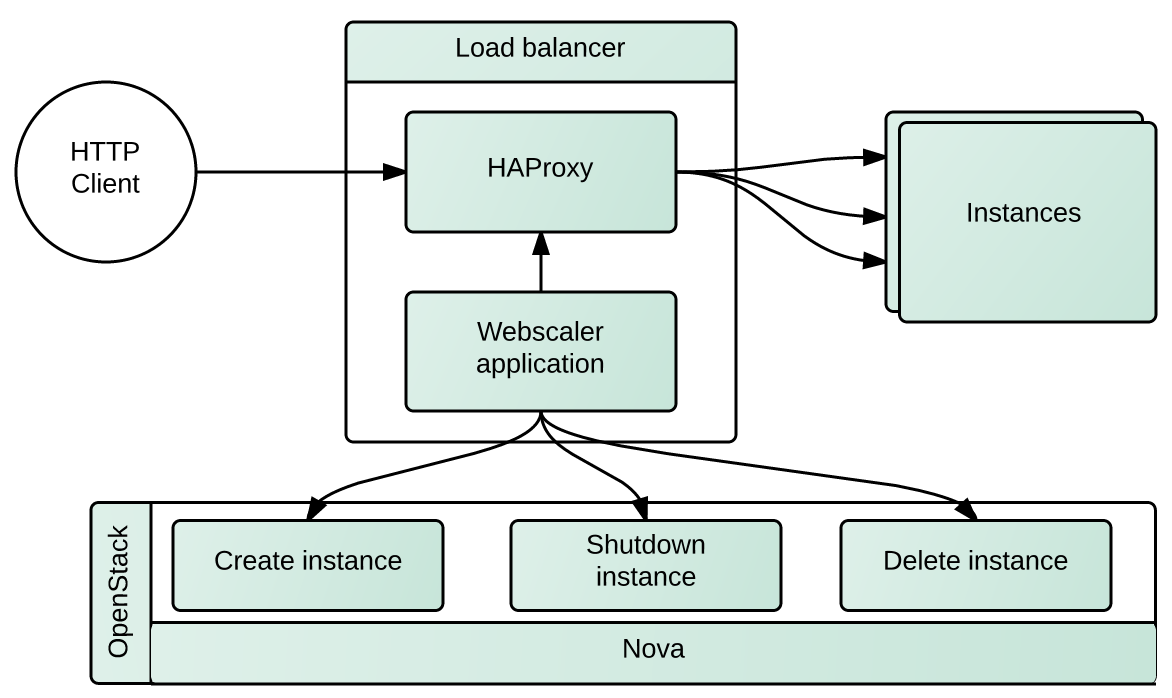
\includegraphics[width=0.8\textwidth]{chapter1/overview}}
\caption{\label{fig:overview}Overview of the setup}
\end{figure}

From the application it will be possible to connect with both the load balancer
and OpenStack, and one requirement for this is that the application must run at
the load balancer instance.



\subsection{OpenStack integration}
OpenStack provides excellent possibilities for integration when programming in
Python. With the use of \textit{python-novaclient} \cite{OpenStackNovaClient} 
it is possible to do almost anything you can do with nova through either the 
CLI or OpenStack Horizon.

It is to be expected that the integration can provide all the needed
functionality of handling the instances. This means that it is possible to
handle the creation of new instances and provide the needed information so that
OpenStack handles the installation of the needed software on the new servers.
This can be done through the usage of cloud-data which is served with a
metadata service provided by OpenStack.

With this the application can scale up completely new instances which is
configured for the service within a short amount of time. When the instances
are no longer needed, the integration can shutdown or delete the instance
altogether.

\subsection{HAProxy}
The integration part to OpenStack is only a small part for administering the
instances to be created, but a way to communicate and get information from
HAProxy is needed. It is possible to get data from HAProxy by issuing commands
to the socket interface. There is also a web interface which provides a
overview of the status of the proxy itself and the stats for each of the
services and backends provided. The interface \vref{fig:haproxy_web_stats} lists
every node and service provided, and shows the different metrics available.

\begin{figure}[htp]
\centering
\makebox[\textwidth][c]{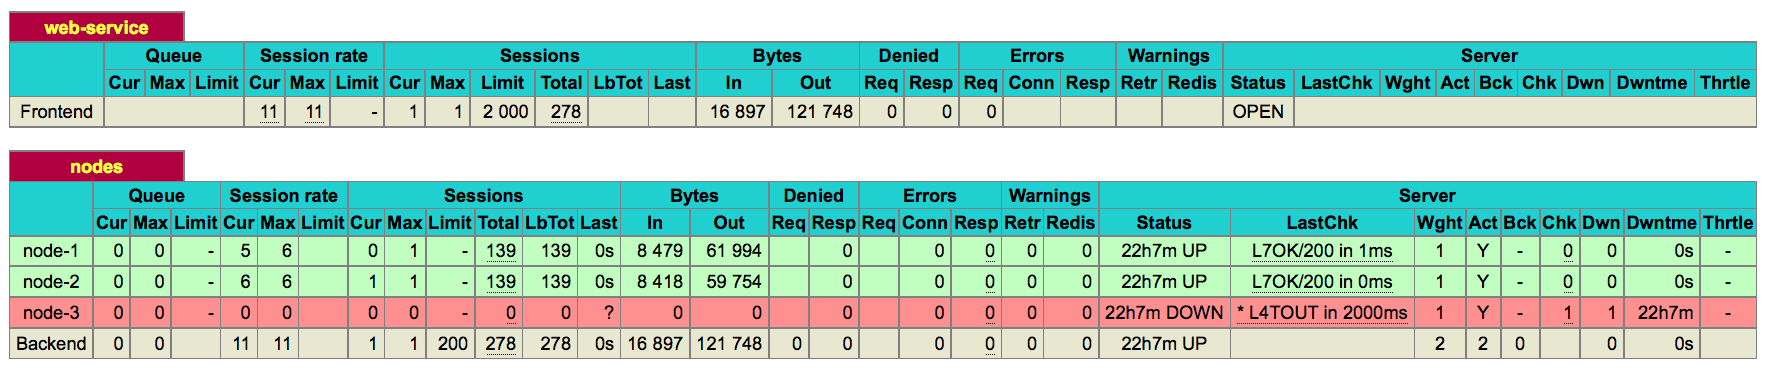
\includegraphics[width=1.3\textwidth]{chapter1/haproxy}}
\caption{\label{fig:haproxy_web_stats}HAProxy web console}
\end{figure}

Everything in this stats page is available from the command line with the use
of a local socket connection to the proxy \ref{haproxy_socat}.

\begin{lstlisting}[label=haproxy_socat,caption=Getting statistics from HAProxy
with sockets,numbers=none]
echo "show stat" | socat /var/run/haproxy/admin.sock stdio
\end{lstlisting}

The socket interface supports many different commands which will be useful to
create a integrated service. This includes setting the backends as
\textit{disable}, \textit{enable} or \textit{draining} which can administer
which backends that should be used. \textit{Draining} mode is specially useful
as what it does is to disable new connection to the proxy, but enables the
existing connections to finish. This is powerful when shutting down backends.

\subsection{Data collection: Acquiring and analysing results}
\label{approach:data}
To enable the scaling there is a need to have a picture of the current state of
service. This is what the load balancer can give with the use of the statistics
given through the socket interface. There are many different metrics to look at
when the goal is to get the rate of user requests. It is possible to get metric
from the web-service, which shows the frontend of the load balancer, or the
backends which can show individual metrics for each backend. The data could be
total transfered bytes, or the more relevant sessions which gives both current
number of sessions for the hole service, or total over time.

For this study the most relevant is the total over time for the service. This
will enable the scaler application to calculate the difference over time and
present it as a rate of incoming requests. This should be done to calculate the
number of requests per second. Thereafter this metric can be used to calculate
the needed servers, when setting a baseline-limit for connections per server
per second.

The difference is then calculated with the following formula:
\begin{equation}
\frac{(newsessions) - (previoussessions)}{sleeptime} =
Sessions/second
\end{equation}

This can then base on the calculation of the needed servers:
\begin{equation}
\frac{ceil(lastdiff)}{server threshold} = needed servers
\end{equation}

This means that there are multiple metrics that need to be stored during the
lifetime of the scaling application.
\begin{itemize}
\item Timestamp
\item Acumulated sessions/requests
\item Difference between last acumulated
\item Needed machines
\item Active machines (Available in OpenStack)
\item Active machines in HAProxy
\end{itemize}

From the data collected it should be possible to show how the scaling is
progressing. The data should therefor be stored in a csv (comma separated)
file so it is possible to import the data into graphing programs, or a
spreadsheet program. Based on this it is possible to generate a picture of how
the process flow is unfolding.

The data could be gathered on a rapid scale, but since it takes time for new
machines to be created or started, this needs to be taken into account. How
rapid the data gathering and scaling should be done is not that important,
since the data will be gathered on an average between the datapoints. A
timeframe of one minute is therefore chosen as it will be enough time to get a
good average, but also enough time for new machines to come up.

\subsection{Simulation for presentation}
To test how the load balancer and the webbalancer application will work during
load, a simulation is needed. The needed function for the simulation is the
possibility to vary the amount of requests to the load balancer. In the first
place the simulation will use httperf to generate load on the load balancer,
but since a variation is needed, this can be implemented by running multiple
httperf. This is implemented as \ref{simulator}.

\lstinputlisting[label=simulator, caption=Simulator of request increased and
descreased, numbers=none]{chapter1/simulator.txt}

With the results presented by the application it will be possible to see a
correlation between the needed scaling of servers based on the incoming http
requests.\\

With this approach it will be possible to create a webscaler by this design
that can scale up new instances in OpenStack based on the number of requests
gathered from HAProxy. It is a reactive design that will scale the machines
after the needed resources. The servicelevel will therefore depend on the
threshold that is set for one server. This is of course a limitation to the
design, and could be resolved by over provisioning or by predicting the needed
level of resources. That would be more of a proactive approach, and not a
reactive approach as this study intends.

\section{Result}
This study presents a implementation of the desired application, that can scale
servers by the incoming rate of web requests. It is totally written in Python,
and uses libraries available to integrate with OpenStack and HAProxy.

The application runs on the load balancer server, as this gives access to the
local socket connection made available by HAProxy. Through this socket
connection the script can communicate with the load balancer and get the
current metrics. This makes the basis for the data that is needed to calculate
the needed amount of web servers.

The program is built to be run continuous, meaning it will always be on. It
could simply be transformed into a service, but at the time being it is
running as a user started application. 

\subsection{Program flow}
The program works with on a few main principles. This is to run every
\textit{60} seconds, and do the calculation to either boot up new servers, or
shut down the existing once. This is done by running a continuous loop, that
every 60 seconds, gathers new performance data from the load balancer. 

\begin{figure}[htp]
\centering
\makebox[\textwidth][c]{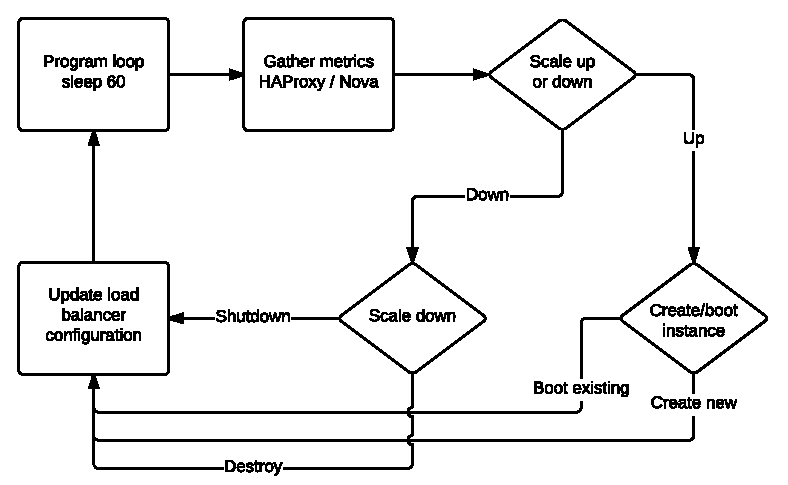
\includegraphics[width=0.9\textwidth]{chapter1/program_flow}}
\caption{\label{fig:program_flow}Program flow}
\end{figure}

As the program runs every minute, it will create an average of the cumulated
web requests on a minute basis. As seen on the figure \ref{fig:program_flow}
this metric allows the application to define what should happen. The different
possibilities are a result of the need of more or less servers. If there are
more servers needed, the application will either start existing shutdown
instances, or create new instances. If there is no need for servers, the
instances will either be shutdown or destroyed. This ensures that the absolute
minimum of needed servers are in action, but at the same time, if the need
arises, an additional instance will be available faster than when creating new
instances.

There are two essential parts of gathering the data. First of all, the
application starts by running two rounds without doing anything. This is to be
able to establish a baseline for what to do. After the baseline is established,
the new metrics are calculated. 

With the gathered metrics a simple calculation can be done to calculate the
need servers. This is shown in the code \ref{needed_servers}, and is an
essential part of the main Webscaler application.

%\newgeometry{margin=2cm}
%\thispagestyle{empty}
% NOTE THAT THE LIMIT FOR A MACHINE IS STATIC AT THIS POINT
\begin{center}
\lstinputlisting[label=needed_servers,caption=Calculation of needed servers,
language=Python,firstline=167,lastline=175]
{chapter1/Webscaler/webscaler.py}
\end{center}
%\restoregeometry

With the code \ref{needed_servers} it is possible to test if there is need for
more or less servers. This is tested in the main loop of the application, that
executes the functions \textit{scale\_up(Needed)} or
\textit{scale\_down(Needed)} according to the amount of
servers that are running in comparison to what is needed.

After the instance count is handled, the load balancer will get an updated
configuration with the new servers.


\subsection{Program structure}
\begin{minipage}[t]{0.7\textwidth}
The program structure is based on a folder structure to create a cleaner
working environment. This means that all the code are separated into a folder
called \textit{bin}, and all the configuration is separated into a folder
called \textit{etc}. The main program \textit{webscaler.py} is at the root of
the application folder alongside the \textit{requirements.txt}. The
requirements file is added to ensure that all the packages needed can be
installed with the use of the package manager \textit{pip} (Python Package
Index). With the combination of virtual environments this application can run
anywhere where Python can run.
This makes it easy to get up and running, with the following four commands:
\begin{Verbatim}[frame=none]
$ virtualenv /path/to/new/environment
$ source /path/to/new/environment/bin/activate
$ pip install -r requirements.txt
(env)$ python webscaler.py
\end{Verbatim}

\end{minipage}
\begin{minipage}[t]{0.3\textwidth}
\dirtree{%
.1 Webscaler.
.2 bin.
.3 haconn.py \ref{lst:haconn.py}.
.3 haproxy.py \ref{lst:haproxy.py}.
.3 hastats.py \ref{lst:hastats.py}.
.3 \_\_init\_\_.py.
.3 nova.py \ref{lst:nova.py}.
.2 etc.
.3 clouddata.txt \ref{lst:clouddata.txt}.
.3 haproxy.cfg \ref{haproxy.cfg}.
.3 openstack.cfg.
.2 README.md.
.2 requirements.txt.
.2 webscaler.py \ref{lst:webscaler.py}.
}
\end{minipage}
The \textit{webscaler.py} file contains the main logic of the scaler
application, see Appendix
~\ref{lst:webscaler.py}:~\nameref{lst:webscaler.py}. This program does not work
without the other files under the \textit{bin} directory. These files include
some central functionality for operating and communicating with the load
balancer and OpenStack. The implementation of this is described in more detail
here.

\subsection{OpenStack integration}
The OpenStack integration uses a module to Python called the
\textit{python-novaclient}. This is built on the same module that is possible
to use from the command line to handle OpenStack nova operations. This
requires a configuration file in the \textit{etc} directory called
\textit{openstack.cfg}. This configuration is a pythonified nova api
configuration, that is supplied by OpenStack that presents the AUTH endpoint
and the user credentials.
This configuration file is read in when the \textit{openstack} class in the
nova.py file is referenced. See \ref{lst:nova.py}:~\nameref{lst:nova.py}.

This code handles all the integration with OpenStack, and provides important
functions like listing the existing instances, shutdown instances, creation of
new instances and operations on them.

To create a new instance there are two possible functions to use, the
\textit{create\_multiple(number)} and \textit{create\_backend()}. The first is
always calling the second function, but can iterate over multiple new
instances, threading each new creation shown in \ref{lst:create_multiple}. The name
is derived from the existing instances, so that the names are human-readable in
the manner of \textit{node-1, node-2, node-3 \dots}. This ensures easy lookup
when debugging, as the nodes will always have the same order, also in the load
balancer.

\begin{center}
\lstinputlisting[label=lst:create_multiple,caption=Nova.py: Creation of multiple instances,
language=Python,firstline=67,lastline=80]
{chapter1/Webscaler/bin/nova.py}
\end{center}

A new instance is created with the function \textit{create\_backend()}
\ref{lst:create_backend}. This
defines all the needed parameters for the new instances to be created.
One of the things that is important to handle when using OpenStack, is the time
it takes after the instance has been created until the IP address is associated
with the new instance. This is done by sleeping while the instance is beeing
built, and after this get the new version.
To prime the new instances the instance is injected with \textit{clouddata}
\ref{lst:clouddata.txt} which is a bash script that installs Apache and PHP.

\begin{center}
\lstinputlisting[label=lst:create_backend,caption=nova.py: Function to create a backend,
language=Python,firstline=84,lastline=119]
{chapter1/Webscaler/bin/nova.py}
\end{center}

The integration is by itself generic, and as long as other cloud solution gives
a supported API or other integration similar to OpenStack, this application is
quite portable. This means that if the python-novaclient library cannot be
used, the only change needed is the nova-openstack python class created in the
\textit{nova.py} file.

\subsection{HAProxy integration}
There are two ways this application works with HAProxy. This is through the
socket connection that are established by the \textit{HAconn.py} file,
\ref{lst:haconn.py}: \nameref{lst:haconn.py}, and with the generation of the
configuration file haproxy.conf, \ref{haproxy.cfg}:\nameref{haproxy.cfg},
located under \textit{/etc/haproxy/haproxy.conf}. This uses the Python template
library \textit{Jinja} to make a template file that can be injected with the
different nodes. This is done since the socket connection to HAProxy not
currently supports adding or removing servers
\cite{haproxy:configuration_manual}.

What the socket connection is perfect for, is to gather metrics and data about
the current status. It is also possible to enable, disable or drain the
instances. This is important, especially the drain mode which makes it possible
to ensure that no connections are lost in mid-transit. When a backend, as the
webserver is called, is in draining mode, no more connections will be
established to the host, but the existing will close when done. This is perfect
when scaling down the amount of servers, and this is done in the
\textit{handle\_scaledown} function in \textit{Webscaler.py}
\ref{lst:webscaler.py}.

In the \textit{hastats.py} the statistical metrics is gathered from HAProxy
socket connection, and parsed to a dictionary. This is what is being used to
find the cumulated requests, that are needed to calculate the needed backends.

\subsection{Output of the \textit{Webscaler}}
In the approach it were specified which metrics were needed to be able to see
that the dynamic scaling application performed as expected \ref{approach:data}.
These data are written every time the application closes, creating a
timestamped file with the gathered data.

\begin{center}
\lstinputlisting[label=lst:data_output,caption=Data
output,language=Python,firstline=1,lastline=2]
{chapter1/webscaler_output.txt}
\end{center}

The output is generated automatic in csv format based on the keys and values in
the list \textit{metrics} which is updated for every run. This does that it is
easy to change the script to write to file for every run, and not just when the
application is done.
The fields describes the following: \\
\begin{table}[h]
\begin{tabular}{ll}
\textbf{Name}   & \textbf{Description}                  \\ \hline
\textbf{diffpt} & Accumulated difference since last run \\
\textbf{haactive} & Active servers in HAProxy \\ 
\textbf{active} & Active servers in OpenStack\\ 
\textbf{epoch} &  Seconds since the script were initiated\\
\textbf{acu} &  Accumulated requests since last load balancer restart\\
\textbf{date} & Date timestamp in ISO format \\
\textbf{diff} & Requests per second in the last time period \\
\textbf{needed} & The amount of servers needed
\end{tabular}
\end{table}

This is the basis of the application, how it gathers the data, and uses the
data and OpenStack to decide and build the new instances. It is built on the
basis that we want a minimum of servers to ensure stability, but also speed
with having sleeping machines. This would be relevant in a ideal world, where
you pay money for the machines you have running, and pay less for the machines
that are shutdown. You are after all still using storage space.

\section{Analysis}
To ensure that the application runs as designed it has been run with the script
described in \ref{approach:data}. This load generating script is meant to
illustrate a rapid growth of webrequests, so that there is a need for more
servers.
The output of the webscaler is the following when this loadtest has finished
\ref{lst:data_output_complete}.

\begin{center}
\lstinputlisting[label=lst:data_output_complete,caption=Data
output,language=Python,firstline=1,lastline=26]
{chapter1/webscaler_output.txt}
\end{center}

The metrics that are displayed \ref{lst:data_output_complete} can be presented 
as a graph where the rate of requests, active servers ,pending servers and the 
needed servers are illustrated fig:~\ref{fig:server_scaling}.

\begin{figure}[htp]
\centering
\makebox[\textwidth][c]{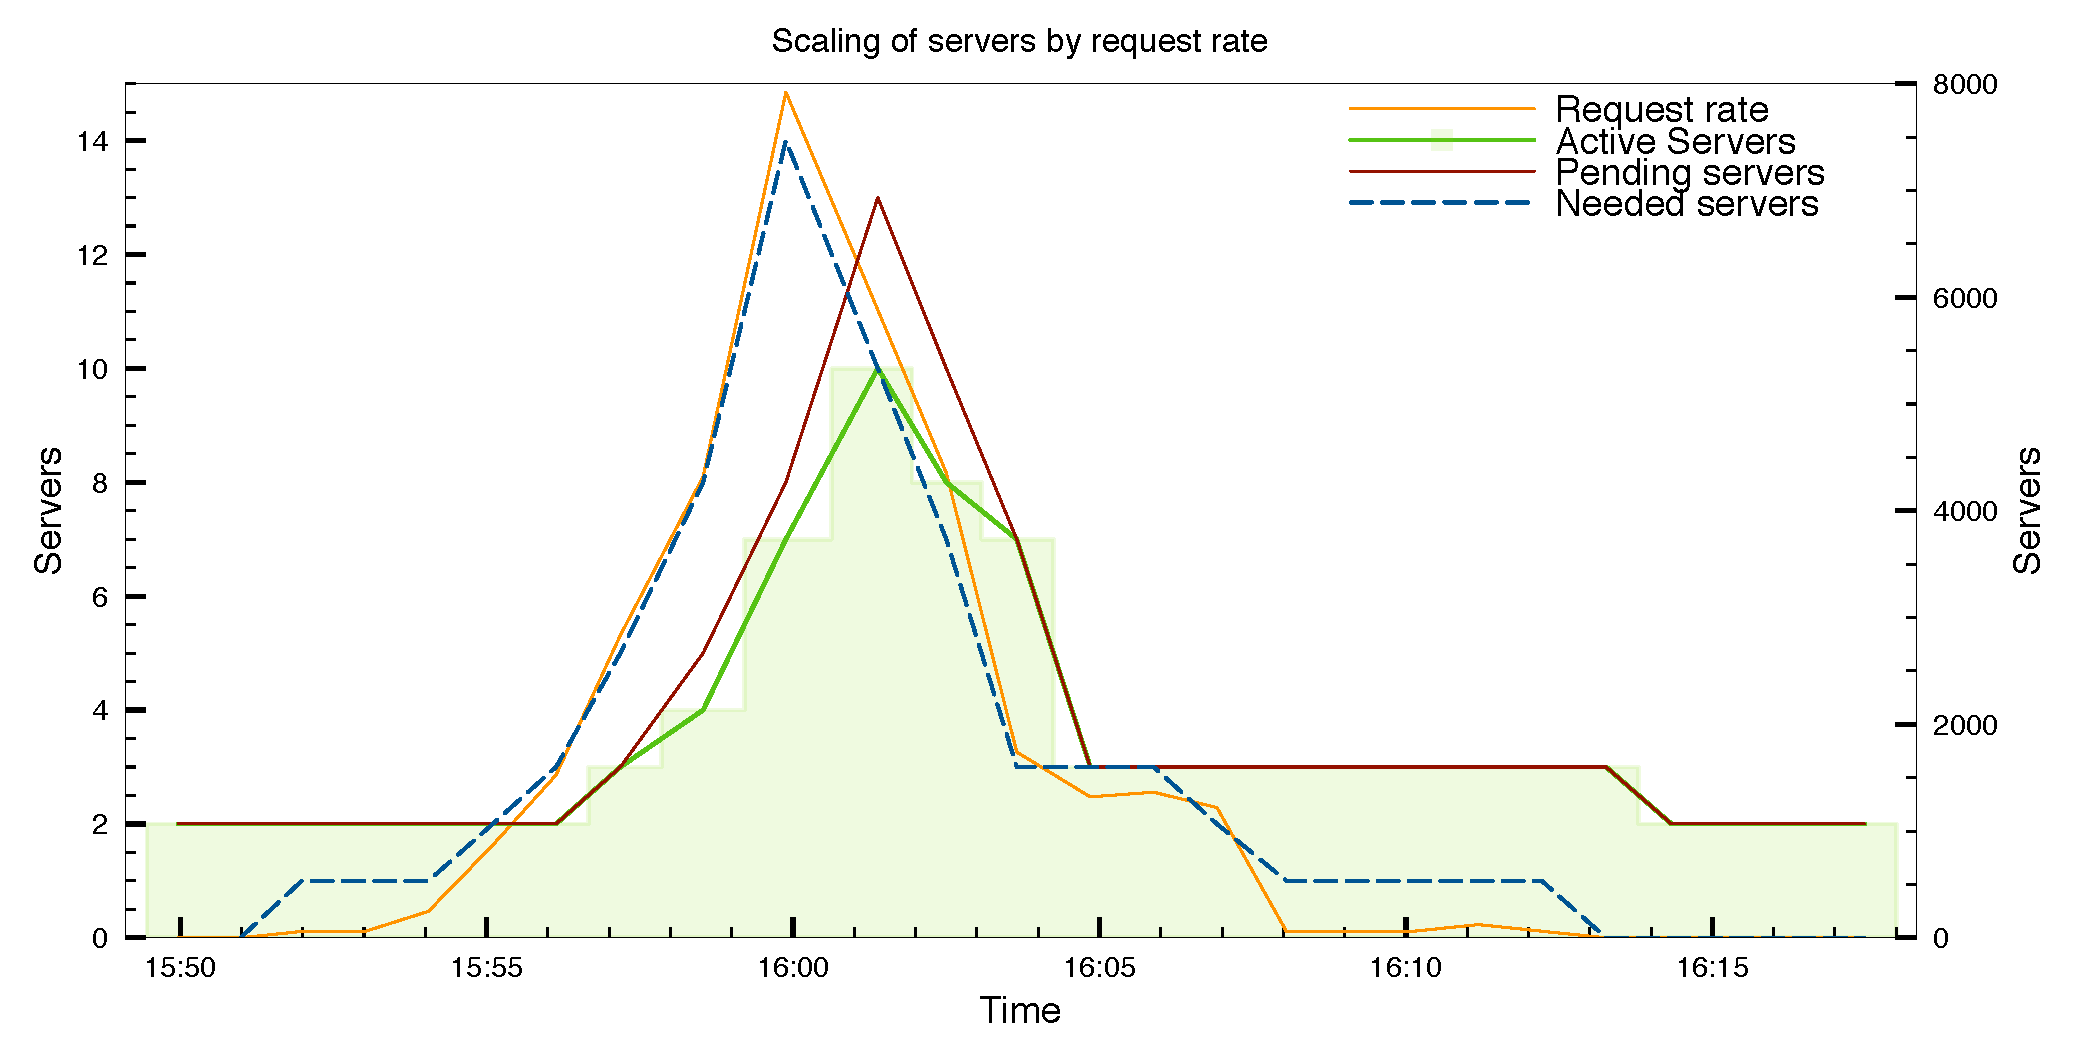
\includegraphics[width=1.25\textwidth]{chapter1/server_scaling_with_requests_legend}}
\caption{\label{fig:server_scaling}Scaling of servers}
\end{figure}

This shows that the scaling algorithm works, and that it can scale up based on
the total number of requests.

\section{Discussion and conclusion}
% Why did i not use MLN
% Reactive handling
% Sometimes slow to respond
% 

\subsection{Improvements}

\subsection{Conclusion}

\section{Appendix}
\newgeometry{margin=2cm}
\thispagestyle{empty}
\begin{center}
\lstinputlisting[label=haproxy.cfg,caption=HAProxy configuration file jinja template]
{chapter1/Webscaler/etc/haproxy.cfg}
\lstinputlisting[label=lst:clouddata.txt,caption=Cloud data injected in
instnace]{chapter1/Webscaler/etc/clouddata.txt}

\lstinputlisting[label=lst:webscaler.py,caption=Webscaler main
application,language=Python]
{chapter1/Webscaler/webscaler.py}
\lstinputlisting[label=lst:nova.py,caption=Nova.py: OpenStack integration,
language=Python]{chapter1/Webscaler/bin/nova.py}

\lstinputlisting[label=lst:haproxy.py,caption=haproxy.py: HAProxy integration,
language=Python]{chapter1/Webscaler/bin/haproxy.py}

\lstinputlisting[label=lst:hastats.py,caption=hastats.py: HAProxy statistical integration,
language=Python]{chapter1/Webscaler/bin/hastats.py}

\lstinputlisting[label=lst:haconn.py,caption=haconn.py: HAProxy socket
connection class,
language=Python]{chapter1/Webscaler/bin/haconn.py}
\end{center}
\restoregeometry
